\ifgerman{\chapter{Implementation}}{\chapter{Implementation}}

This chapter describe in detail about how data was collected, what preprocessing techniques were applied to the data in order to make it fit for machine learning algorithm to learn from, how data was resampled in order to balance it to some extent, how it was clustered and what are the details of the architecture of the models and what are the evaluation strategies applied.

\section{Data Collection}

To begin with the implementation, the first step was to obtain the data. Obtaining the data was particularly  challenging as these summaries were frequently changing, so scraping the data at different times results in different assignment of a single document in different categories. Also another challenge was that when documents for English and German were scraped separately, it happened quite often that some of the documents from one of the language were missing. Due to these challenges, a carefully crafted scraper which scrapes the data only if the documents from both of the languages are available, this in turn added a time overhead.

For scraping the data, Python library \textit{urllib}\footnote{https://docs.python.org/3/library/urllib.html} is used, this scraps the HTML data out of the desired web page. Then Python library \textit{Beautiful Soup}\footnote{https://www.crummy.com/software/BeautifulSoup/bs4/doc/} is used on the data collected from the web pages to parse the HTML content and produce simple text documents. During the parsing of the data, the corresponding label of the document was also parsed in order to complete the training dataset. First, the title of the document was scraped. Then all the HTML elements of the web page are removed to construct the text document. A new folder with name of the category that is the label of document is then used to store the documents of that class and each document is given the corresponding title as the name of the file.

\section{Data Cleaning}\label{preprocessing}

The preprocessing involved removing of \textit{punctuation's}, \textit{numbers}, \textit{currency symbols} as they do not contribute anything in the classification process. The next step is to normalize the text, this step is necessary because of the \textit{inflection} added due to the modification of words.

%\todo{A figure explaining how played, plays and playing is all from the root word \textit{play} }
Stemming and Lemmatization are two techniques used to normalize the text. Both techniques reduces words to its root form. Stemming reduces the word into base but this base may or may not be the morphological root of the word. It should suffice that the related words are mapped to the same base, even if the base is not a valid root. For example, words \textit{argued}, \textit{arguing}, \textit{argue} and \textit{argues} will all be stemmed to \textit{argu}, even though the base \textit{argu} is not a valid term in itself. The process of stemming is more heuristic. It removes affixes such as \textit{-ed,-ize, -s,-de} without taking into account that the base might not be a word in the same language. On the contrary lemmatization reduces the words by ensuring that the base belong to the language. The base word in lemmatization is called a \textit{lemma}. Lemmatization is necessary in the cases where it is necessary to get valid words. This is the reason, that instead of stemming, lemmatization is used as word normalization technique. 

\begin{table}[!ht]
\centering
\begin{tabular}{ccc}
\hline
\textbf{Words} & \textbf{Stemming} & \textbf{Lemmatization} \\ \hline
argue & argu & argue \\ 
arguing & argu & argue \\ 
argued & argu & argue \\ 
argues & argu & argue \\ \hline
\end{tabular}
\captionsetup{justification=centering,margin=2cm}
\caption{Comparison of word normalization techniques, stemming and lemmatization}
\label{table:StemVSLemma}
\end{table}

As the last step, \textit{stop words} from both the languages were removed because, because they don't contribute anything, and also they increase the training time of the algorithm. For German language, \textit{umlauts - ä, ö and ü} are converted into its base form that is \textit{ä to ae, ö to oe and ü to ue.}

Following are the steps in which the preprocessing was done.

\begin{enumerate}
    \item As a first step, \textit{stop words} are removed.
    \item Next step is to lemmatize the words.
    \item Removal of other unnecessary symbols are removed. For example, § is symbol of paragraph and is extensively used in legal text. • is also another example.
    \item Remove numbers
    \item Punctuation 
    \item Conversion of umlauts to its base form.
\end{enumerate}

The order of the steps is also important as it will help in reducing the overload on some of the processes. For example, when the stop words are removed in the first step, then the lemmatizer would not have to go through those words and that will decrease the time taken to process the text. There were other Unicode characters which were also removed.

For removing the stop words Python library \textit{NLTK}\footnote{https://www.nltk.org/} (Natural Language Toolkit) is used. It provides stop words in both English and German language. To lemmatize the words \textit{spaCy}\footnote{https://spacy.io/} library is used for both the languages. To remove unnecessary symbols, custom functions were written. Number removal and conversion of umlauts were also done using custom functions.

\iffalse


\subsection{Data Preprocessing for pretrained word embeddings}
Pretrained word embeddings are generated using larger corpora, hence they can be used for variety of task in natural language processing. These models are trained on corpora that have no specific domain. Legal text is different from the corpora these models are trained on such that the some words we find in legal text are rarely used outside the legal domain. 

Facebook's MUSE multilingual word embeddings \cite{conneau2017word} were trained on large corpus \ref{backgroundCrosslingual}. These word embeddings are created by learning a mapping between the two sets of monolingual word embeddings.\todo{have to write what methods were used to create these} The monolingual word embedding used in were created using fastText \cite{bojanowski2017enriching}. These pretrained vectors were trained on Common Crawl and Wikipedia Coprus. There was no preprocessing involved except for lower casing the words. Hence, to use these word embeddings, I need to use the corpus with only lower case words and avoid all the preprocessing mentioned in the section in order to have the classifier learn better. If the preprocessed data is used with the embedding that were created using non processed data then even if the 

\fi
\section{Data Resampling} \label{dataResampling}
The EUR-Lex summaries, are the summarised versions of legislations. These summaries are written in an abstract manner to apply for multiple situations, so that one regulation may belong to several categories. Multi-label classifier with very few examples might not be applicable as the classifier will favour majority class because of the imbalance. 

From \ref{graph:distribution of data english docs} it is clear that the data suffers from class imbalance. To mitigate the problem of class imbalance we upsample minority class or downsample majority class. In our case, upsampling minority class is difficult as it is very hard to produce alike documents because of nature of text and downsampling minority class would lessen the already less data. We had to find a way to not only downsample the majority in such a fashion that would result into balancing the data as well as not lessen the data to an extent that is not useful anymore.

As the data is multilabeled it can be exploit because of the fact that a sample might belong to more than one class. The documents are transformed in such a way that if a document belongs to two or more class, then it will be kept in the class with minimum number of samples. That is the class label for that document will be the one with the fewest examples. This method will downsample the majority class as only the duplicated documents are removed from it but also make this classification problem a multi-class from a multi-label one. In the testing phase, the predictions are allowed from the set of all the true labels. This method however introduces a bais towards the minority classes but it acknowledges the presence of other possible category assignment in the end result.

\begin{figure}[!ht]
\begin{center}
\makebox[2pt]{
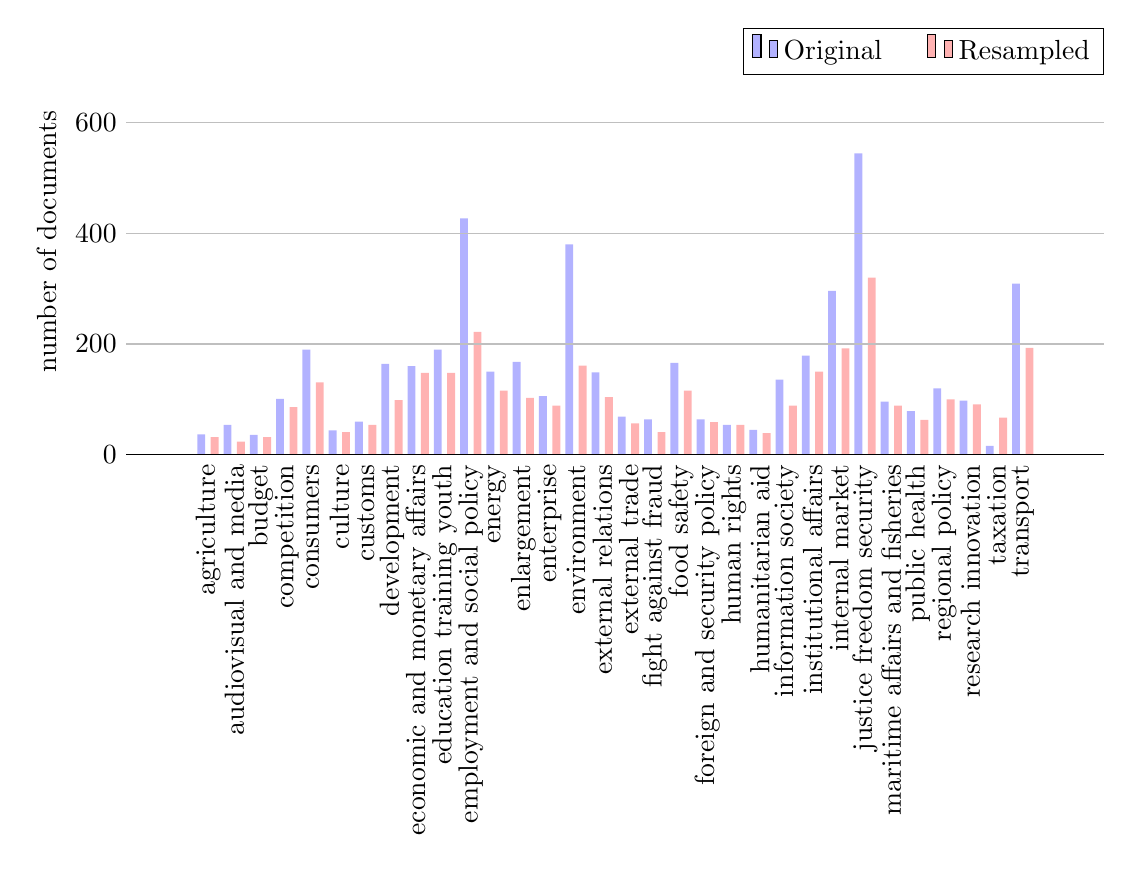
\begin{tikzpicture}
  \centering
  \begin{axis}[
        ybar, axis on top,
        title={},
        height=7cm, width=14cm,
        bar width=0.1cm,
        ymajorgrids, tick align=inside,
        enlarge y limits={value=.1,upper},
        ymin=0, ymax=700,
        axis x line*=bottom,
        axis y line*=left,
        y axis line style={opacity=0},
        tickwidth=0pt,
        ytick style={draw=none},
        enlarge x limits=true,
        legend style={
            at={(1,1)},
            anchor=north east,
            legend columns=-1,
            /tikz/every even column/.append style={column sep=0.5cm}
        },
        ylabel={number of documents},
        symbolic x coords={
        agriculture,
        audiovisual  and  media,
        budget,
        competition,
        consumers,
        culture,
        customs,
        development,
        economic  and  monetary  affairs,
        education  training  youth,
        employment  and  social  policy,
        energy,
        enlargement,
        enterprise,
        environment,
        external  relations,
        external  trade,
        fight  against  fraud,
        food  safety,
        foreign  and  security  policy,
        human  rights,
        humanitarian  aid,
        information  society,
        institutional  affairs,
        internal  market,
        justice  freedom  security,
        maritime  affairs  and  fisheries,
        public  health,
        regional  policy,
        research  innovation,
        taxation,
        transport
        },
       xtick=data,
       x tick label style={rotate=90,anchor=east},
       %nodes near coords={\pgfmathprintnumber[precision=0]{\pgfplotspointmeta}}
    ]
    \addplot [draw=none, fill=blue!30] coordinates {
        (agriculture, 37)
	    (audiovisual and media,54) 
		(budget,36) 
		(competition,101) 
		(consumers,190) 
		(culture,44) 
		(customs,60) 
		(development,164) 
		(economic and monetary affairs,160) 
		(education training youth,190) 
		(employment and social policy,427)
		(energy,150)
		(enlargement,168)
		(enterprise,106)
		(environment,380)
		(external relations,149)
		(external trade,69)
		(fight against fraud,64)
		(food safety,166)
		(foreign and security policy,64)
		(human rights,54)
		(humanitarian aid,45)
		(information society,136)
		(institutional affairs,179)
		(internal market,296)
		(justice freedom security,544)
		(maritime affairs and fisheries,96)
		(public health, 79)
		(regional policy,120)
		(research innovation,98)
		(taxation,16)
		(transport,309)  };
   \addplot [draw=none,fill=red!30] coordinates {
      (agriculture, 32)
(audiovisual and media, 24)
(budget, 32)
(competition, 86)
(consumers, 131)
(culture, 41)
(customs, 54)
(development, 99)
(economic and monetary affairs, 148)
(education training youth, 148)
(employment and social policy, 222)
(energy, 116)
(enlargement, 103)
(enterprise, 89)
(environment, 161)
(external relations, 104)
(external trade, 57)
(fight against fraud, 41)
(food safety, 116)
(foreign and security policy, 59)
(human rights, 54)
(humanitarian aid, 39)
(information society, 89)
(institutional affairs, 150)
(internal market, 192)
(justice freedom security, 320)
(maritime affairs and fisheries, 89)
(public health, 63)
(regional policy, 100)
(research innovation, 91)
(taxation, 67)
(transport, 193) };
\legend{Original, Resampled}
\end{axis}
\end{tikzpicture}
}
\end{center}
\captionsetup{justification=centering,margin=2cm}
\caption{Class distribution of the EUR-Lex summaries corpus, comparing the original
to the resampled distribution.}
\label{graph:originalVSresampled}
\end{figure}


\section{Clustering} \label{clustering}
Document cluster in information retrieval helps in organization, extraction of topic and text, filtering. The idea here was that given the number of classes and the number of documents per classes as it is a unbalanced dataset,it will be difficult for a classifier to learn on this data. 

Clustering of documents was only possible provided that all the documents $d$ of a category $C$ belong only to that category. Also, it is important to find out what is the number $n$ that the documents must be clustered into. The number of clusters $n$ is determined bu silhouette score \cite{rousseeuw1987silhouettes} and elbow analysis \cite{thorndike1953belongs}. 

K-Means cluster is used here to cluster the documents. Splitting the documents this way, the number of classes to be predicted by each classifier is reduced thus, resulting in specialization advantage for each classifier. However, the final classification depends on the classification from previous classifiers, so any error introduced will be propagated downwards. This method of division is can be advantageous as we have $32$ classes and it can be a challenge for a single classifier to learn on them given the amount of data.

The \ref{} shows the cluster assignments of all the 32 categories of the EUR-Lex summaries.

\begin{table}[!ht]
\centering
\begin{tabular}{cc}
\hline
\textbf{Class Label} & \textbf{Cluster Assignment} \\ \hline
Agriculture & 1 \\ 
Audiovisual and Media & 1 \\ 
Budget & 2 \\ 
Competition & 1 \\ 
Consumers & 1 \\ 
Culture & 2 \\ 
Customs & 2 \\ 
Development & 2 \\ 
Economic and Monetary Affairs & 2 \\ 
Education Training Youth & 2 \\ 
Employment and Social Policy & 1 \\ 
Energy & 1 \\ 
Enlargement & 2 \\ 
Enterprise & 1 \\ 
Environment & 1 \\ 
External Relations & 2 \\ 
External Trade & 2 \\ 
Fight Against Fraud & 2 \\ 
Food Safety & 1 \\ 
Foreign and Security Policy & 2 \\ 
Human Rights & 2 \\ 
Humanitarian Aid & 2 \\ 
Information Society & 1 \\ 
Institutional Affairs & 2 \\ 
Internal Market & 1 \\ 
Justice Freedom Security & 2 \\ 
Maritime Affairs and Fisheries & 2 \\ 
Public Health & 1 \\ 
Regional Policy & 2 \\ 
Research Innovation & 2 \\ 
Taxation & 1 \\ 
Transport & 1 \\ \hline
\end{tabular}
\caption{Assignment of EUR-Lex summaries into clusters}
\label{table:ClusterAssignments32Classes}
\end{table}


\section{Training the Word Vectors}

The model used in creation of the word vectors is a neural network, and neural networks are data hungry as it requires a lot of data to train them properly. As a result, another domain specific dataset is used in this experiment because dataset used for classification is small. Hence, the whole EUR-Lex dataset was used as it contains 19,348 documents mostly consisting regulations, decisions and directives of European Union \cite{jf:SemanticLaw}.

\subsection{Training Cross Lingual Word Embedding}\label{implementationCrossLingual}

I will be using the technique suggested by Duong et. al \cite{duong-EtAl:2016:EMNLP} (see \ref{backgroundCrosslingual}).
The dataset used for creating a domain specific word embeddings is the EUR-Lex dataset, as the dataset used for classification (EUR-Lex summaries) is less compared to the EUR Lex dataset. For creating bilingual dictionary, \textit{EuroVoc} thesaurus \cite{steinberger2002cross} provided by Publication office of European Union will be used. It is available in 24 official languages recognised by European Union. This thesaurus is domain specific hence it does not involve common words that might occur in the documents. Due to this reason, this thesaurus is combined with bilingual dictionaries that are available from \textit{Facebook MUSE} \cite{conneau2017word}. This bilingual dictonaries were created using Facebook's internal translation tools. The authors claims that these dictionaries handle the polysemy of the words better. This combined bilingual dictionary with the original EUR-Lex dataset was used to create the legal domain specific bilingual word embeddings. 

For creating General purpose word embedding, Facebook's MUSE python library \cite{conneau2017word} (see \ref{backgroundCrosslingual}) is used, first English and German language word vectors are obtained from Facebook's Fasttext library and then MUSE library align them in a single vector space, after the alignment both the vectors can be combined to be used for classification purpose. 


\section{Architecture and Training}
This section describes in detail the specifics of architectures of the algorithm used for all the three questions mentioned in \ref{sec:conceptRQ}.

Before beginning to train the models, it is necessary to divide the dataset into a training set and a testing set. Generally, 70\% of the data is for training purposes, and 30\% to evaluate the model. This division is stratified, which means that the class distribution in training, and testing set will remain almost equal. The stratified division ensures that there are enough examples for each class in training, and test phase of the model. 

Neural network based classification models are prone to \textit{overfitting} \cite{Prechelt1998}. Overfitted model will perform well on the training data but fail to perform well on the testing data. To put it simply, the error on the training set will keep on decreasing while the error on the unseen data starts getting worst. To avoid this situation regularization techniques such as Dropout, L1 and L2 regularization and early stopping is used.

Dropout and L1, L2 regularization are explicit regularization technique, that is it explicitly reduces the model complexity. In Dropout regularization techniques, during the training, a fraction of randomly selected neurons are ignored. Hence, their activation contribution to the forward pass and weight updates are removed. While Dropout regularization reduces the model complexity by removing randomly selected neuron during training, L1 and L2 regularization reduces the model complexity by imposing penalty to the weight of all the features and features with non zero weights respectively.      

On the other hand early stopping regularization is implicit which does not affect the complexity of the model directly \cite{zhang2016understanding}. Early stopping, monitors the training process and halts it once the performance of the model starts degrading. It does so by monitoring validation data. 


Dropout, L2 regularization and early stopping can be configured in \textit{keras} while building the model. During the training we split 30\% of training data for validation purpose so that there is no need for splitting validation data at the time when we split the dataset into training and testing.

\subsection{Question 1} \label{impQuestion1}

In the first research question Support Vector Machines are compared to Bidirectional LSTMs. When using an SVM algorithm we do not know beforehand the value of $C$ (See \ref{sec:svm}). To find that out, we need some kind of selection mechanism must be done. The aim is to find out the value of $C$ such that it can predict accurately on unknown data. One method of finding the value of $C$ is called \textit{Grid Search Cross Validation} (Grid Search CV). This method is straight forward, first we select the a number of values of $C$, then we divide the training set into $n$ equal sized subsets. Then we train the SVM using one value from $C$ on the $n-1$ subset and predict using 1 subset that left, we repeat this process until each and every instance of the training set is predicted once and for every value of $C$.

This process is computationally expensive as each subset will be trained on every value of $C$. We used the following values of $C$ (0.001,0.01, 0.1,1,10,100) and found 1 to be preforming better.

To train SVM, TF-IDF matrix of the English corpus is created using the \textit{sklearn}\footnote{https://scikit-learn.org/stable/} python library and then this TF-IDF matrix is used to train a linear SVM with the $C$ value of 1 for the same \textit{sklearn} library. 

The SVM is compared against two Bidirectional LSTM models, one without clustered data on single language (English) and one with clustered data (English and German). The data used for training both SVM and Bidirectional LSTM is different, while SVM is trained on whole documents, Bidirectional LSTMs are trained on sentences created using sliding window technique (see \ref{backgroundSlidingWindow}, \ref{question1}). The \ref{fig:PlainLSTM} shows the architecture of the Bidirectional LSTM model trained on English corpus with all the 32 classes. The Bidirectional LSTM models were created using \textit{Keras}\footnote{https://keras.io/} python library. 

The hyperparameter for Bidirectional LSTM training on English corpus without clustered data is listed in \ref{table:hyperparameterLSTM32class}. 

\begin{table}[!ht]
\centering
\begin{tabular}{cc}
\hline
\textbf{Hyperparameter} & \textbf{Value} \\ \hline
Sentence Size & 30 words \\
Batch Size & 32 \\
Embedding Dimension & 200 \\
Hidden 1 Size & 40 \\
Hidden 2 Size & 40 \\
Dropout 1 & 0.5 \\
Dropout 2 & 0.5 \\
$l2$ regularization 1 & 0.04 \\
$l2$ regularization 2 & 0.01 \\
Learning Rate & 0.001 \\ \hline
\end{tabular}
 \captionsetup{justification=centering,margin=2cm}
\caption{Hyperparameter of Bidirectional LSTM for training English language corpus without clustered data}
\label{table:hyperparameterLSTM32class}
\end{table}


\begin{figure}[!ht]
    \centering
    \includegraphics[width=9cm, height=12cm]{pics/EN_32.png}
    \captionsetup{justification=centering,margin=2cm}
    \caption{Architecture of Bidirectional LSTM for training English language corpus without clustered data}
    \label{fig:PlainLSTM}
\end{figure}
\clearpage
The hyperparameter for the Bidirectional LSTMs used on clustered data is exactly similar to the one without clustered data trained on English laguage \ref{table:hyperparameterLSTM32class}

The architecture for Bidirectional LSTM trained on cluster 1 and cluster 2 data is shown in \ref{fig:cluster1&2LSTM}



\begin{figure}[!ht]
    \centering
    \includegraphics[width=9cm, height=12cm]{pics/LSTM_LEGALEMB_CLUSTER_1.png}
    \captionsetup{justification=centering,margin=2cm}
    \caption{Architecture of Bidirectional LSTM for training English and German language corpus on cluster 1 and cluster 2 data}
    \label{fig:cluster1&2LSTM}
\end{figure}


\clearpage

\subsection{Question 2}
In the second question general purpose embeddings, Facebook's MUSE is compared to word embeddings created using EUR-Lex corpus (see \ref{implementationCrossLingual}).

Both the approaches using the general purpose resource and the domain specific resources, uses Bidirectional LSTMs trained on clustered data, similar to the Bidirectional LSTMs in \ref{impQuestion1}
The hyperparameters for the both approaches is listed in \ref{table:FBMuseGeneralpurpose} for general purpose embeddings and \ref{table:DomainSpecificHyperparameter} for domain specific embeddings.

\begin{table}[!ht]
\centering
\begin{tabular}{cc}
\hline
\textbf{Hyperparameter} & \textbf{Value} \\ \hline
Sentence Size & 30 words \\
Batch Size & 32 \\
Embedding Dimension & 300 \\
Hidden 1 Size & 40 \\
Hidden 2 Size & 40 \\
Dropout 1 & 0.5 \\
Dropout 2 & 0.5 \\
$l2$ regularization 1 & 0.04 \\
$l2$ regularization 2 & 0.01 \\
Learning Rate & 0.001 \\ \hline
\end{tabular}
\captionsetup{justification=centering,margin=2cm}
\caption{Hyperparameter of Bidirectional LSTM for training on English and German language with clustered data using general purpose word embedding created using Facebook's MUSE python library}
\label{table:FBMuseGeneralpurpose}
\end{table}

\begin{table}[!ht]
\centering
\begin{tabular}{cc}
\hline
\textbf{Hyperparameter} & \textbf{Value} \\ \hline
Sentence Size & 30 words \\
Batch Size & 32 \\
Embedding Dimension & 200 \\
Hidden 1 Size & 40 \\
Hidden 2 Size & 40 \\
Dropout 1 & 0.5 \\
Dropout 2 & 0.5 \\
$l2$ regularization 1 & 0.04 \\
$l2$ regularization 2 & 0.01 \\
Learning Rate & 0.001 \\ \hline
\end{tabular}
\captionsetup{justification=centering,margin=2cm}
\caption{Hyperparameter of Bidirectional LSTM for training on English and German language with clustered data using domain specific word embedding created from EUR-Lex dataset}
\label{table:DomainSpecificHyperparameter}
\end{table}

The only difference between the training parameters of both the approaches is the embedding dimensions, the general purpose embedding are in 300 dimensions whereas the domain specific embedding are in 200 dimensions. The reason for this difference is that while aligning two embeddings in a single vector space is a computationally inexpensive task, then learning the embedding from scratch for two languages. Decreasing the dimensions will result in the reduction of training time and hence the dimension of domain specific word embeddings are 100 less than general purpose embeddings.

The architecture for Bidirectional LSTM trained using general purpose word embeddings is shown in \ref{fig:FBMuseCluster} and Bidirectional LSTM trained using domain specific word embeddings is show in \ref{fig:LegalEmbCluster}.

\begin{figure}[!ht]
    \centering
    \includegraphics[width=9cm, height=12cm]{pics/FBMUSE_Untrained_cluster_1.png}
    \captionsetup{justification=centering,margin=2cm}
    \caption{Architecture of Bidirectional LSTM for training English and German language corpus on cluster 1 and cluster 2 data using general purpose embeddings created using Facebook MUSE python library}
    \label{fig:FBMuseCluster}
\end{figure}



\begin{figure}[!ht]
    \centering
    \includegraphics[width=9cm, height=12cm]{pics/LSTM_LEGALEMB_CLUSTER_1.png}
    \captionsetup{justification=centering,margin=2cm}
    \caption{Architecture of Bidirectional LSTM for training English and German language corpus on cluster 1 and and cluster 2 data using general purpose embeddings trained on EUR-Lex dataset}
    \label{fig:LegalEmbCluster}
\end{figure}

For evaluating the predictions, each document is divided into sentences using the same sliding window technique used to create the training data, then predictions are stored for every sentence of a document and the predictions are summed up and the class with highest value is considered the class of the document. 

\subsection{Question 3}
The third question evaluates the capability of training multiple languages in a single Bidirectional LSTM model compared to training different models for different languages. For this purpose two models one for the English and another for German language will be compared to a single model trained on both the English and the German language together.

Training on the clustering data will only be performed in the case where both the languages are used in a single model, this is due the fact that performing clustering on a single language will reduce the number of samples in each cluster significantly. So for this question one model with both the languages will be trained without clustering and one with clustering. 

The hyperparameters and architecture for all the models will be same to ensure fair comparison. The hyperparameters are for this question is listed in \ref{table:hyperParameterQuestion3} and the architecture for this question is shown in \ref{fig:architectureQuestion3}

\begin{table}[!ht]
\centering
\begin{tabular}{cc}
\hline
\textbf{Hyperparameter} & \textbf{Value} \\ \hline
Sentence Size & 30 words \\
Batch Size & 32 \\
Embedding Dimension & 300 \\
Hidden 1 Size & 40 \\
Hidden 2 Size & 40 \\
Dropout 1 & 0.5 \\
Dropout 2 & 0.5 \\
$l2$ regularization 1 & 0.04 \\
$l2$ regularization 2 & 0.03 \\
Learning Rate & 0.001 \\ \hline
\end{tabular}
\captionsetup{justification=centering,margin=2cm}
\caption{Hyperparameters of Bidirectional LSTM for training on the English and the German language with and without clustered data and trained on both languages separately}
\label{table:hyperParameterQuestion3}
\end{table}

\begin{figure}[!ht]
    \centering
    \includegraphics[width=9cm, height=12cm]{pics/Question3.png}
    \captionsetup{justification=centering,margin=2cm}
    \caption{Architecture of Bidirectional LSTM for training on the English and the German language with and without clustered data and trained on both languages separately}
    \label{fig:architectureQuestion3}
\end{figure}

The evaluation of all the above mentioned questions is in the following chapter.